\chapter{Background}

\section{Image Quality Assessment}

As portrayed in the introduction, image quality assessment (IQA) is vital for many applications, but on the other hand is hard to achieve as such because of its reliance on the quantification of human perception. 
The most solid approach to embrace IQA is through subjective assessments, but this is not practical in real-life applications since users can’t always be dependent upon to comment on the perceived quality. 
On the other hand, objective image quality assessment focuses on implementing human perception models that can estimate the quality of an image as perceived by a person based solely on pixel analysis information.

In the following, we briefly review current subjective quality assessment methods to then go deeper in the state-of-the-art of methods for objective quality assessment.

\subsection{Subjective image quality assessment}

Subjective image quality assessment methods use human observers to express their personal opinion on the quality of images which are used to be assessed. 
Because humans are the end users in a large portion of the multimedia applications, subjective IQA methods are the most reliable and accurate for image quality assessment.

Several international standards have been proposed for performing subjective image quality assessment such as , ITU P913 \cite{ITU2014}, ITU P910 \cite{ITU-TRecommendationP.9102008} and ITU BT 500 \cite{Bt2002}. 
The main objective of subjective IQA methods for a given set of images is to assign a score to each of them that quantifies the perceived quality of the user. In most cases, a scaling process can be achieved, either explicitly or implicitly.

Subjective testing usually focuses on quantifying average observer's perceived quality. 
A group of subjects is requested to evaluate an image and give its perceived quality score.
These scores are then accumulated and the final score is calculated to reflect the quality perceived by an average observer. 
For the calculation of this final score, different scales could be used, for example, direct scaling in which the perceived quality of an image is calculated as the mean of the scores assigned to that image by each subject. (Mean Opinion Score (MOS) or Differential Mean Opinion Score (DMOS)). 
The objective IQA methods (to be followed) are intended to use different models to predict these mean values.

Despite being the most accurate and reliable, subjective IQA methods are highly impractical for real-world applications as it is very expensive and time-consuming to gather an adequate number of observers to evaluate image quality. Consequently, more practical objective IQA methods are used for many applications.

\subsection{Objective image quality assessment}

Rather than using human observers, objective IQA methods are aimed at using relevant models that can predict image visual quality as perceived by humans. Because these algorithms require no human observer, they are fast and very practical for many applications in the real world, such as image enhancement, image restoration, etc.

To estimate the perceptual quality of the given image (called test image), either in the presence or absence of its reference image, most of the objective IQA methods share a common framework of three main phases as illustrated in Fig.\ref{fig:obj-fw}. These
three phases are described in the following

\begin{figure}[H]
  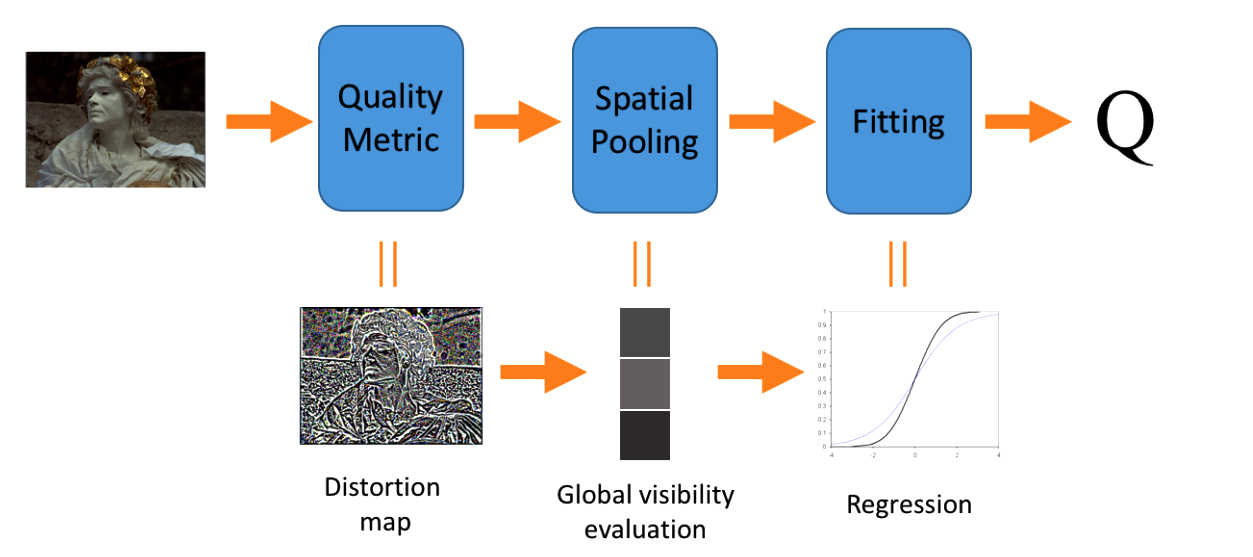
\includegraphics[width=\linewidth]{figures/objective-framework.png}
  \caption{General Objective image quality assessment framework}
  \label{fig:obj-fw}
\end{figure}

\begin{enumerate}
  \item The test image is processed pixel by pixel or region by region in accordance with the objective IQA method used to measure the amount of distortion present in it. This phase then outputs the distortion measured in the form of a distortion map containing the image quality local description. This step is equivalent to the feature extraction. 
  \item A multidimensional phase is produced in the first phase, but humans perceive image quality as a single global entity rather than the local properties of an image. A spatial pooling strategy is generally used to downsample the multidimensional distortion map to a single quality score in order to produce a global quality assessment. \cite{Wang2006}
  \item Since in the first two phases non-linearity, which characterizes perception, is not used, the output may not be sufficiently accurate. Thus, to increase the overall accuracy of the framework, an appropriate strategy could be applied. This requires a set of images along with their subjective quality scores (obtained through subjective testing), and a parametric model whose parameters are learned through the analysis of image model predictions and their actual subjective scores through regression. This learned model is then used to transform predicted scores into better estimates allegedly consistent with human perception. 
\end{enumerate}

Objective IQA strategies are classified into three large categories.

\subsubsection{Full-reference image quality assessment (FR-IQA)}

FR-IQA methods aim to achieve objective IQA goals while taking as input both reference and test images. Because these algorithms also require reference images to estimate visual quality, their scope is limited to a few applications where reference images are easily available, such as compression of images and watermarking. 

Over time, a lot of FR-IQA algorithms were proposed. According to one of these methods, image quality can be computed as a peak-signal-to-noise ratio (PSNR), which is simply a ratio of a signal's maximum power and distortion power. The distortion power is generally calculated to calculate the pixel-wise difference between the reference and the distorted image in terms of mean-square-error (MSE). PSNR has the advantages of being simple and very inexpensive computationally, but it does not deliver very good performance because the essential physiological and psychophysical characteristics of the human visual system (HVS) are not included in this algorithm. 

Another FR-IQA algorithm, the Structural Similarity Index (SSIM) \cite{Wang2004}, advances FR-IQA from raw pixels to structures. It is based on the assumption that HVS is highly adapted to extract structural information present in an image, and degradation of images is perceived as a change in this structural information. SSIM therefore aims to evaluate the quality of an image by measuring variations in the structural information of distorted images (in relation to their reference image). In evaluating the perceptual quality of images, SSIM has been shown to outperform PSNR 

Another lately proposed FR-IQA \cite{Zhang2011} algorithm is the Function Similarity Index (FSIM). It is based on the fact that HVS uses low-level features to understand images (like edges and zero crossing). FSIM uses two features to estimate an image's quality: a primary feature called Phase Congruency, which is a contrast-invariant dimensionless measure of the local structure's significance, and an image gradient magnitude feature. FSIM shows superior performance on different datasets than PSNR and SSIM algorithms. 

Recently, Bosse \emph{et al.} \cite{Bosse2018} presents an IQA data-driven approach based on deep neural networks. The network consists of 10 convolution layers and 5 pooling layers for extraction of features, and 2 fully connected layers for regression, making it significantly deeper than related IQA models. Unique features of the proposed architecture are that I it can be used in a no-reference (NR) as well as in a FR-IQA setting with slight adaptations and (ii) it enables joint learning of local quality and local weights in a unified framework, i.e. the relative importance of local quality to the global quality estimate. 

\subsubsection{Reduced-reference image quality assessment (RR-IQA)}

RR-IQA methods aim to achieve objective IQA goals by estimating the quality of the test image while using partial reference image information. Usually this partial information is in the form of features extracted from the images of the reference. 

In communication networks, RR-IQA finds its application that is used to transmit images and videos. Using RR-IQA algorithms, partial reference image information transmitted through these communication networks can be used to track visual quality degradation of images and videos transmitted. In similar applications, therefore, RR-IQA algorithms are preferred over FR-IQA algorithms as presented in \cite{Atsawaraungsuk2015, Redi2010}.

\subsubsection{No-reference image quality assessment (NR-IQA)}

NR-IQA methods are intended to achieve the objectives of objective IQA by using only test images to estimate the quality of the image. Due to the lack of information on reference images, these methods are considerably more challenging than FR-IQA and RR-IQA. But due to their application in the wide variety of fields, they are also more desirable, ranging from image processing to image enhancement, where reference images are usually not available. NR-IQA methods are also used in a wide range of online applications, such as communication systems, image acquisition systems, etc. \cite{Chandler2013}, making it very important for them to be computationally cheap. 

Some early NR-IQA attempts used distortion-specific methods that approach IQA tasks by using models very specific to a specific type of distortion. These methods are more specific to applications where there is prior knowledge of the type of distortion. For example, in an application to measure quality losses in compressed images, knowledge of the appearance of compression artifacts, such as blocking and ringing, could be used to design NR-IQA methods that can detect their visibility 

It is more useful to have algorithms, regardless of the types of distortion, that can be applied for general purpose NR-IQA. Existing NR-IQA approaches for general purposes could be further divided into two broad categories: Natural scene statistic based approaches (NSS) and Feature learning based approaches


\subsection{IQA in Visual Data Compression}

\begin{figure}[H]
  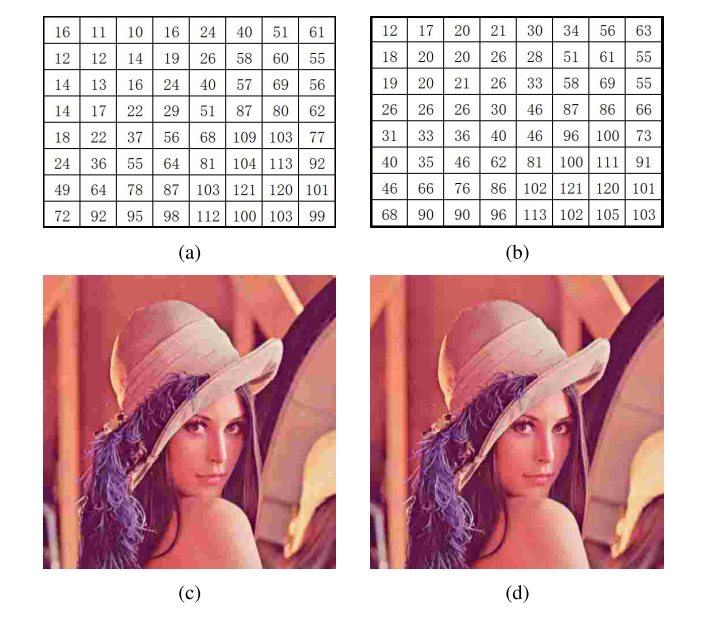
\includegraphics[width=\linewidth]{figures/jpeg.png}
  \captionsetup{justification=raggedright}
  \caption{Examples of quantization table and the corresponding compressed
    JPEG images.} 
  \label{fig:jpeg}
  \subcaption*{(a) JPEG default quantization table at quality factor equal to
    50; 
    \newline(b) Optimized quantization table with the optimization goal of MS-SSIM; \newline(c) JPEG image using default quantization table at QF = 10, 0.234 bbp,
    PSNR = 30.45, SSIM = 0.819, MS-SSIM = 0.946; \newline(d) JPEG image using
    MS-SSIM optimized quantization table, 0.226 bpp, PSNR = 30.49, SSIM = 0.818, MS-SSIM = 0.953}
  
\end{figure}

While the bitstream has been normalized by image coding standards, different coding parameters or modes determined by different IQA metrics will obviously result in distinct compression performance. In JPEG, the custom quantization table is one of the optional coding parameters, and the default table is empirically determined based on human perception \cite{Wallace1992}. For example, in Fig.\ref{fig:jpeg}(a), which is scaled to generate quantization tables for other quality factors, the quality factor (QF) quantization table of the luminance component equal to 50 is shown. In addition to the standard JPEG quantization table, the open source and well-optimized JPEG codec, \emph{libjpeg}, has adopted another 8 quantization tables, one of which is an optimized MS-SSIM-based quantization table as shown in Fig.\ref{fig:jpeg}(b). 

In \cite{Ratnakar2000}, the researchers proposed optimization of the image-dependent quantization table based on the signal fidelity-based metric, MSE, which achieved substantial bit rate savings at the same quality as PSNR. However, because of the poor correlation between perceptual quality and PSNR, these optimization strategies can not ensure the same visual quality improvement. The researchers introduced SSIM and its variants into image and video coding in \cite{Channappayya2008}, \cite{Wang2012} and \cite{Ou2011} to optimize the process of rate distortion, but the performance improvement is not yet so satisfying. The upper and lower boundaries of the average SSIM index were derived for the first time by Channappayya \emph{et al.}\cite{Channappayya2008} as a function of the quantization rate for different source distributions, e.g. uniform, Gaussian and Laplacian. Wang \emph{et al.}\cite{Wang2012} used SSIM as the quality metric for optimizing rate distortion instead of MSE and achieved a bit rate saving of about 5\%-10\% compared to the original H.264/AVC. Ou \emph{et al.} \cite{Ou2011} applied SSIM to the problem of perceptual rate control with a gain of 0.008 SSIM (corresponding to a saving of 14\ percent bitrate). We can see from this work that the improvements in quality are still small. 

Essentially, with regard to the compression of the perceptual image, although different encoding optimization strategies can improve the image quality at the same bit rate level, the quality fluctuations are usually limited within a small range. However, most traditional IQA databases contain only coarse-grained compression distortion levels, and IQA algorithms on the fine-grained quality prediction for image compression problem can not be evaluated well. For example, the scaled quantization tables in Fig.\ref{fig:jpeg}(a) and \ref{fig:jpeg}(b), respectively, compress the JPEG images in Fig.\ref{fig:jpeg}(c) and \ref{fig:jpeg}(d) at similar bitrates. Although the image shows less blocking artifacts in Fig.\ref{fig:jpeg}(d), it has a lower SSIM value but higher PSNR and MS-SSIM values than the image shown in Fig.\ref{fig:jpeg}(c). These different IQA algorithms show opposite quality rankings on the level of fine-grained distortion, which motivates us to re-examine existing IQA algorithms and examine their suitability to distinguish fine-grained distortions 

\section{Neural Networks}

\subsection{Artificial Neural Network}

Artificial Neural Network (ANN) is not a brand new idea. It was first introduced as a computational model of "nerve net" in the human brain by Warren McCulloch and Walter Pitts \cite{McCulloch1943} in 1943. After that, the concept and architecture of neural networks are further developed by follow-up researchers. Neural networks have long been constrained by hardware performance. The advancement in GPU design and brain science led to a boom in the development of neural networks only in recent decades. 

\begin{figure}[H]
  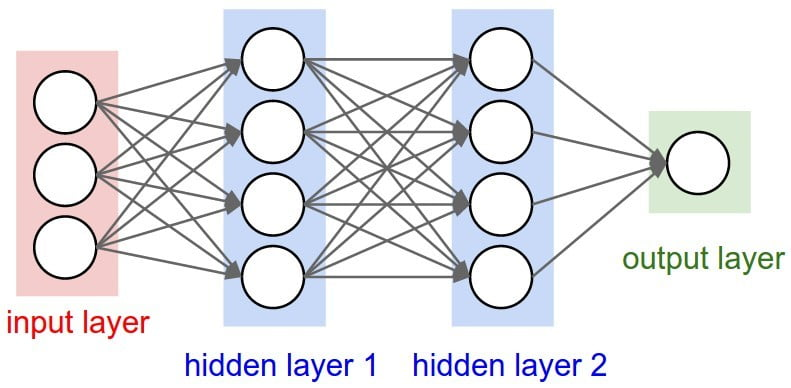
\includegraphics[width=\linewidth]{figures/ann.jpg}
  \caption{The basic structure of Neural Network.}
  \label{fig:ann}
\end{figure}

A common modern neural networks consist of a large number of nodes called neurons. Each neuron does a simple calculation, usually $y = Wx + b$, where $W$ is called Weight and $b$ is called Bias. The neurons form multiple layers and the result value $y$ of each neuron is then passed to the neurons in the next layer. The first layer is called input layer as shown in Fig.\ref{fig:ann}. As its name implies, it takes features from outside the network as input. The last layer is output layer and its output value is the prediction given by the neural network.

\subsection{Training Neural Network}

First, Weight Metric and Bias Metric are initialized with random values (or pre-trained value obtained from other benchmark data). A training of the neural networks is required to adjust those parameters to fit into a particular task.

Back-propagation (BP) \cite{Rumelhart1986} is known as the most common and popular method of training neural network. The objective of back-propagation is to compute the partial derivative, or gradient, $\frac{\partial E}{\partial w}$ of a loss function E with respect to any weight w in the network. The loss function
$E$ calculates the difference between prediction of neural network and its expected output, after one or a batch of sample data go through the network. A loss function is usually defined as:

\begin{equation} \label{eq:lossabs}
E=\frac{1}{N}\sum_{i=1}^{N}|f(x_i)-y_i| 
\end{equation}

or

\begin{equation} \label{eq:losssqr}
E=\frac{1}{N}\sum_{i=1}^{N}(f(x_i)-y_i)^{2} 
\end{equation}

where $f(x)$ is the equivalent function fo the neural network. Equation \ref{eq:lossabs} is called $L1$ loss while equation \ref{eq:losssqr} is called $L2$ loss. In practice, $L2$ loss is the most popular one due to the fact that it is more sensitive to examples that are far away from expected output. 
Thus the trained neural network is hopefully more general. 
On the other hand, $L1$ loss is not that sensitive to a minority of output that is far from the expectation and takes care of the average error of the majority. 
It is particularly useful if training data is not collected very carefully and may contain incorrect samples.

Thus the progress of training by BP can be presented as:

\begin{enumerate}
  \item Feed forward one batch of training data through the neural network
  \item Calculate the loss between ground truth and output
  \item Back-propagate the network and calculate the partial derivative, or gradient, $\frac{\partial E}{\partial w}$
  of loss function $E$ with respect to each weight $w$ in the network
  \item Update the weights in the network according to loss, gradient and learning rate (LR)
  \item Repeat step 1 to 4 until training is complete, usually when the number of cycles set by researcher is reached or the loss value is lower than a threshold
\end{enumerate}

This method is called \enquote{back-propagation} partly because the partial derivative is calculated using chain rule:

\begin{equation}
\frac{\partial E}{\partial w_{ij}} = \frac{\partial E}{\partial o_j} \frac{\partial o_j}{\partial wsum_j} \frac{\partial wsum_j}{\partial w_{ij}}
\end{equation}

where $E$ is the loss function, $w_{ij}$ is the weight from neuron $i$ to neuron $j$, $o_j$ is the output of the neuron $j$, $wsum_j$ is the weighted sum of outputs to neuron $j$ from the previous layer.

From the output layer to the input layer, we can calculate them one by one and use the results in later layers to calculate the former layers. Therefore, when doing backwards, calculating partial derivatives is actually quite cheap.

A neural network with multiple layer structure has proved its power on image recognition \cite{Rowley1998}. However, it suffers from \enquote{the curse of dimensionality} heavily. It means that the number of parameters in the network goes up quickly when the dimension (resolution) of input image increases. Early neural networks work on low resolution images such as $20 \time 20$ and $32 \time 32$. Early benchmark datasets, MNIST \cite{LeCun1998} and CIFAR10 \cite{Krizhevsky2009} for instance, are also collections of small images with $20 \time 20$ and $32 \time 32$ pixels. At that time, neural networks can take care of those images with hundreds or thousands of parameters. When the size of target image rise to around $200 \time 200$, an input layer with 40000 neurons is needed. Assuming the first hidden layer is fully connected and has the same number of neurons as the input layer, which is quite common in practice, at least $40000 \time 40000$ individual parameters is needed in just 2 layers. The mass of parameters not only consumes computing resources, but also causes serious overfitting problems. 

Overfitting means that a statistical model tries to describe each sample of training instead of finding regular patterns in the collection of samples. Fig.\ref{fig:overfit} shows a simple case of overfitting. The regression function tends to "remember" each sample's distinctive characteristics individually but fails to determine the trend of all samples. Although it passes every sample point with 0 loss, it does not generalize the unseen data. Even a linear function can predict better than it. 

\begin{figure}[H]
  \centering
  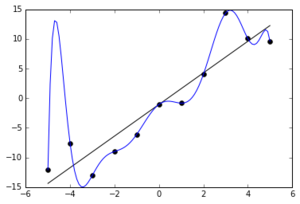
\includegraphics[width=.7\linewidth]{figures/overfit.png}
  \caption{The function overfit the train samples.}
  \label{fig:overfit}
\end{figure}

Overfitting usually occurs when there are too many parameters in the neural network compared to the number of training samples, allowing the network to easily remember all samples. To limit the number of parameters in neural network, researchers find a way to reuse parameters in various parts of the image, which is a Convolutional Neural Network (CNN).

\subsection{Convolutional Neural Network}

CNN is a type of neural network designed specifically for image recognition. The architecture of CNN inspires from the organization of human visual cortex. Fig.\ref{fig:cnn} shows the basic structure of a convolutional neural network. $X_{i,j}$ represents the pixels in the input image. $A$ is the kernel of the first convolutional layer and is repeatedly used on each block of four pixels. The neurons on the second layer then takes the outputs of the first layer as their inputs and use the same kernel $B$. Fig.\ref{fig:kernel} shows the mapping between 2 layers. One blocked in the front layer, which is a  $m \times n \times d_1$ tensor ($m = n$ in most cases), is multiplied by a $m \times n \times d_1 \times d_2$ kernel and mapped to a $1 \times 1 \times d_2$ block in the next layer. The $m \times n \times d_1$ block in the front layer is called receptive field, which means all neurons in such block is connected to one neuron in the next layer, and their information is gathered together by a neuron in next layer.

\begin{figure}[H]
  \centering
  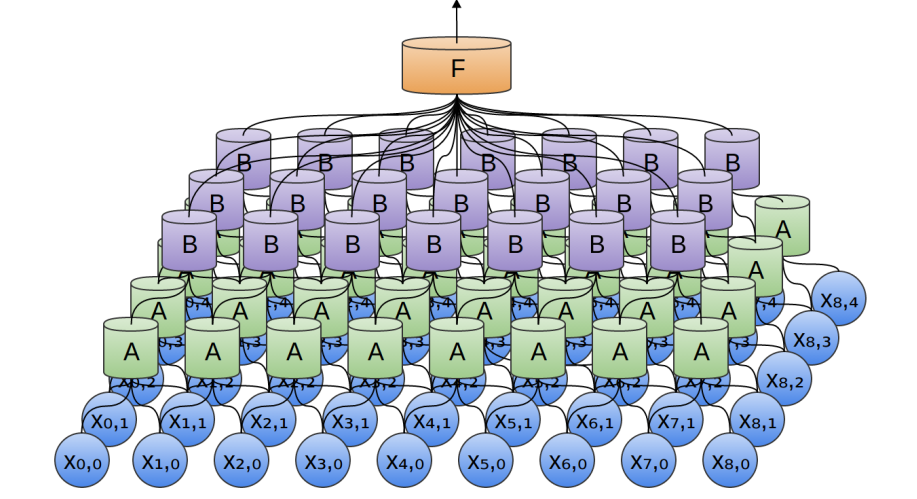
\includegraphics[width=\linewidth]{figures/cnn.png}
  \caption{CNN share the kernel on each layer.}
  \label{fig:cnn}
  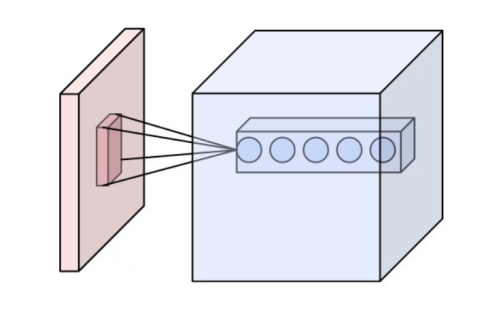
\includegraphics[width=0.5\linewidth]{figures/kernel.png}
  \caption{Kernel that maps $m \times n \times d_1$ block in the previous layer to an $1 \times 1 \times d_2$ block in next layer.}
  \label{fig:kernel}
\end{figure}

CNN is proved to be very efficient in pattern recognition and other image classification tasks. Its superior performance comes from some particular features. The most important feature is perhaps its spatial invariant. Since the same kernel is used repeatedly in the whole input space, it can detect its corresponding pattern no matter where the pattern shows up. This feature significantly reduces the number of patterns the network needs to learn. 

Another important feature is its ability of abstracting and concentrating information. In Fig.\ref{fig:cnn}, each neuron $A$ (instance of kernel) on first layer accesses information from 4 pixels. On the second layer, each neuron $B$ connect to 4 neurons in the first layer, which means it can access information gathered from 9 pixels in the input image. As the network goes deeper, the neurons in later layers get access to larger area of the input image. At last, at the final layer, the network gets an overall abstract sense of the input image. All of these concentration and abstract procedure are learned automatically by back-propagation. It is still a mystery to researches that how those things exactly happen because the mid product of hidden layers are really difficult to understand by human beings.

\textbf{ReLU Layers} 

ReLU layers usually stand between 2 convolutional layers. ReLU stands for Rectified Linear Units. ReLU layer applies the non-saturating activation function to the outputs of convolutional layers:

\begin{equation} \label{eq:relu}
f(x) = max(0,x)
\end{equation}

ReLU layers are very simple but they efficiently add nonlinear properties to the decision
making function of the overall network as well as the sigmoid function:

\begin{equation} \label{eq:sigmoid}
f(x) = \frac{1}{1+e^{-x}}
\end{equation}

and the hyperbolic tangent function:

\begin{equation} \label{eq:hypo}
f(x) = \tanh(x)
\end{equation}

\begin{figure}[H]
  \centering
  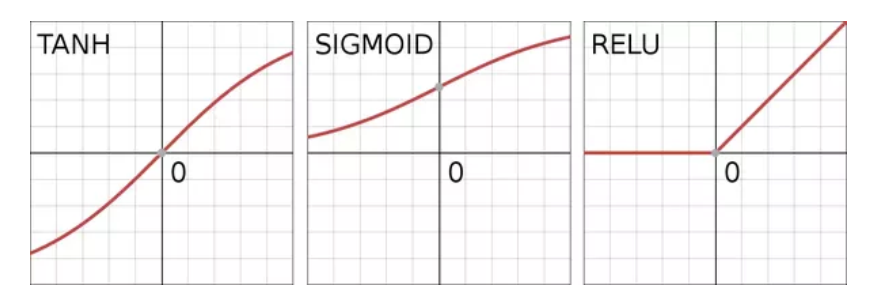
\includegraphics[width=\linewidth]{figures/activation.png}
  \caption{Common nonlinear functions used in CNN: ReLU, Sigmoid and hyperbolic tangent.}
  \label{fig:activation}
\end{figure}

Fig.\ref{fig:activation} shows the response of 3 methods. The 3 methods share the same idea of inhibiting negative outputs and amplifying/keeping positive outputs of the early layers, which is a simulation of how human brain cells work. Hyperbolic tangent function and sigmoid function are widely used in old models but ReLU function becomes more preferable recently because it is proved to be much computational cheaper without making any significant differences in accuracy \cite{Krizhevsky2012}.

\textbf{Pooling Layers} 

\enquote{Pooling} is a nonlinear down-sampling method widely used in CNNs. Fig.\ref{fig:pool} shows a common max pooling layer with a $2 \times 2$ filter size and a stride of 2. The filter move through the entries with a certain stride, pooling layer maps each block in former layer to a single value. Pooling layer concentrates the information in former layer and provides the later layers a larger \enquote{vision} in the original image. Also, pooling helps reducing the number of parameters in the network and hence has an effect of overfit control. The most popular pooling methods are max pooling and min pooling, where the filter takes the max or min value in each block as the output. Average pooling, which uses the average of all values in the block as output is also commonly used in old days. However, it has given its place to max pooling since the later one is proved to work better in practice \cite{Scherer2010}.

\begin{figure}[H]
  \centering
  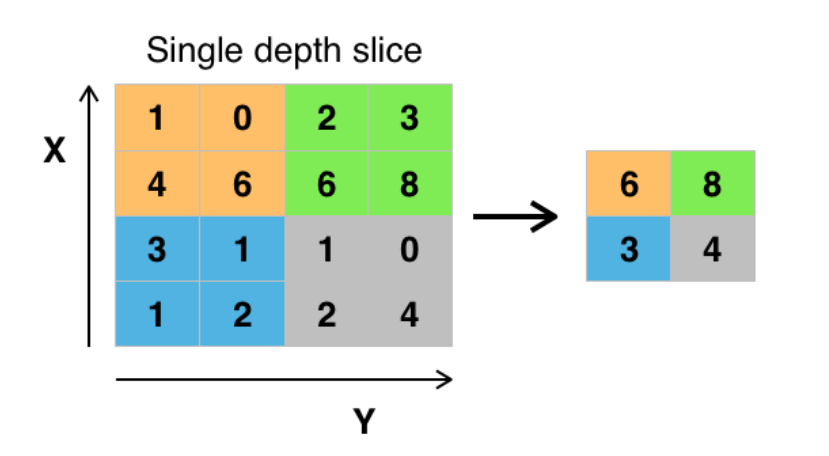
\includegraphics[width=\linewidth]{figures/pooling.png}
  \caption{A max pooling layer with a $2 \times 2$ filter size and a stride of 2}
  \label{fig:pool}
\end{figure}